\documentclass[12pt, twoside]{article}
\usepackage[francais]{babel}
\usepackage[T1]{fontenc}
\usepackage[latin1]{inputenc}
\usepackage[left=10mm, right=10mm, top=7mm, bottom=7mm]{geometry}
\usepackage{float}
\usepackage{graphicx}
\usepackage{array}
\usepackage{multirow}
\usepackage{amsmath,amssymb,mathrsfs} 
\usepackage{soul}
\usepackage{textcomp}
\usepackage{eurosym}
\usepackage{lscape}
 \usepackage{variations}
\usepackage{tabvar}
 
\pagestyle{empty}

\title{\ul{\textbf{Agrandissement et r�duction}}}
\date{}

\begin{document}
\maketitle

\ul{D�finitions}: On consid�re deux figures $\mathcal{F}_1$ et $\mathcal{F}_2$
telles que toutes les longueurs de la figure $\mathcal{F}_2$ sont obtenues en
multipliant celles de la figure $\mathcal{F}_1$ par un m�me nombre k
strictement positif.

$\bullet$ Si \textbf{k est sup�rieur � 1}, on dit que la $\mathcal{F}_2$ est un
\textbf{agrandissement de facteur k} de la figure $\mathcal{F}_2$.


$\bullet$ Si \textbf{k est inf�rieur � 1}, on dit que la $\mathcal{F}_2$ est un
\textbf{r�duction de facteur k} de la figure $\mathcal{F}_1$.

\bigskip 

\bigskip 


\ul{Remarque}: Le facteur k est aussi appel� \textbf{coefficient} ou
\textbf{rapport} d'agrandissement ou de r�duction.


\bigskip


\bigskip 

\ul{Propri�t�s}: Si une figure $\mathcal{F}_1$ est un agrandissement ou une
r�duction d'une figure $\mathcal{F}_2$ alors:


$\bullet$ les longueurs de la figure $\mathcal{F}_2$ sont
\textbf{proportionnelles} � celles de la figure $\mathcal{F}_1$;

$\bullet$ les mesures des angles, le parall�lisme et la perpendicularit� sont
\textbf{conserv�s}.


\bigskip 

\bigskip 

\ul{Exemple}:


\begin{center}
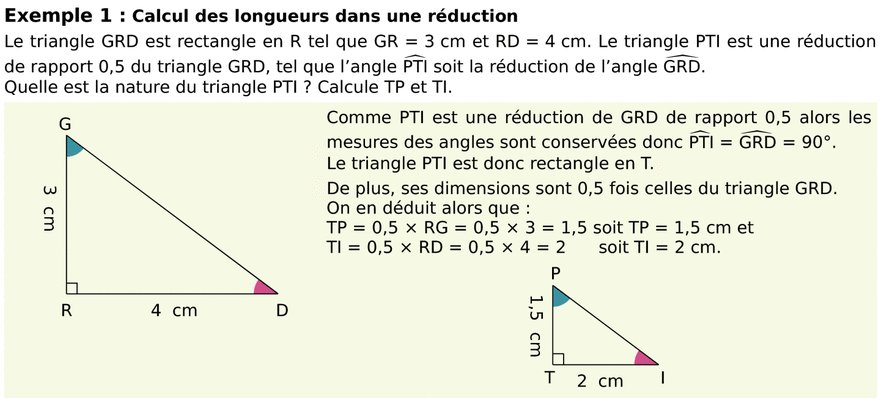
\includegraphics[width=18cm]{images/exemple1.jpg}
\end{center}




\bigskip


\ul{Propri�t�:} Dans un agrandissement ou une r�duction de rapport k:

$\bullet$  le p�rim�tre d'une figure est multipli� par k,

$\bullet$ l'aire d'une figure est multipli�e par $k^2$,

$\bullet$ le volume d'une figure est multipli� par $k^3$.



\bigskip


\ul{Exemple:} Aire du triangle GRD: $\dfrac{3 \times 4}{2}=6 cm^2$.


PTI est une r�duction du triangle GRD de rapport 0,5 donc l'aire du triangle
PTI vaut: $0,5^2 \times 6=1,5cm^2$

\end{document}
